\chapter{Úvod}

V současné době v domácnostech stále přibývají inteligentní elektrická zařízení se zabudovaným operačním systémem. Počítače a chytré telefony jsou již téměř samozřejmostí, inteligentní televize a ledničky se pomalu přidávají. Tato zařízení jsou ovládána lidmi s různou dovedností. Koncept dynamicky vyvažované obtížnosti se snaží o přizpůsobování systému uživatelům dle jejich schopností.

Tématem této diplomové práce je dynamicky vyvažovaná obtížnost(DDA) v počítačových hrách. DDA v počítačových hrách má za úkol přizpůsobovat hru hráči, aby z ní měl co nejlepší požitek. 

V úvodní kapitole popisuji cíl práce, blíže zadefinuji koncept DDA a jeho dělení do kategorií. Dále ve stručnosti zmíním různé aplikace DDA nejen v komerčním průmyslu, ale také např. v lékařství a ve vzdělávání.

V druhé kapitole se zaměřím na pojem zábava, představím pojem flow a zadefinuji několik možných metrik, pomocí kterých lze zábavu měřit. Ve chvíli, kdy jsme schopni zábavu měřit, můžeme nejen ohodnocovat zábavu po skončení hry, ale můžeme tyto metriky dále použít při dynamické úpravě her.

Třetí kapitola je rešerší existujících DDA přístupů. Mezi existujícími přístupy jsou zástupci známých oblastí umělé inteligence jako jsou neuronové sítě, genetické algoritmy, POMDP, fuzzy logika, teorie her a další.

Na začátku čtvrté kapitoly  popíši teoretický základ z teorie her a jejích algoritmů, který poté využiji při návrhu vlastního přístupu DDA nazvaného hráčem prostředí. Představím zde 4 algoritmy založené na novém principu.

Navržené algoritmy je potřeba otestovat. V páté kapitole seznamuji s testovacím prostředím a použitými hrami v něm.

V předposlední šesté kapitole popisuji provedené experimenty a jejich výsledky.

V závěru shrnuji provedenou práci, jestli se podařilo splnit zadání a cíle diplomové práce.

Nakonec přidávám v příloze stručný popis ovládání aplikace a několik dodatečných grafů z experimentů, které se nehodily do šesté kapitoly.

\section{Cíl diplomové práce}

Cílem diplomové práce je prozkoumat možnosti přístupů k dynamické adaptivitě v počítačových hrách, navrhnout přístup nový a ten analyzovat a porovnat s přístupy existujícími.

\section{Definice}

Dynamické vyvažování obtížnosti (dynamic difficulty adjustement, DDA) je obecným konceptem, jak přistupovat k návrhu programů, jež jsou využívány uživateli rozdílných schopností a zkušeností. 

Klasickým přístup je předdefinování několika rozdílných nastavení s odlišnými požadavky na dovednosti uživatelů, kteří si mezi těmito nastaveními volí ručně. Naopak dynamický, adaptivní přístup volbu nastavení nechává alespoň z části na samotném programu, který se rozhoduje na základě modelu uživatele. Dále se zaměřím na koncept DDA používaný v počítačových hrách.

Synonymy pro DDA jsou např. dynamic difficulty balancing, dynamic game balancing, auto-dynamic difficulty, adaptive difficulty. Vyvažování obtížnosti je základem velké většiny her využívající DDA. Myšlenka za tím je jednoduchá. Je-li hra pro hráče příliš snadná, hráč se nudí, hru opustí. Naopak je-li hra příliš obtížná, hráč je frustrován, hru opouští. V obou případech hra ztrácí své uživatele.

Hlavní cílem DDA v počítačových hrách je udělat hru více zábavnou pro hráče. Míra zábavnosti hry není závislá pouze na její obtížnosti. Jak lze definovat zábavu a jak ji lze měřit více popíši v kapitole \ref{sec:defzab}. 

Každé využití auto-dynamického vyvažování hry lze zařadit do několika kategorií z různých úhlů pohledu. Různé hry vyžadují různé přístupy a je dobré se zamyslet nad konkrétní hrou. Vybrat si z jakých kategorií by mělo být DDA použito. Designér hry by si měl položit několik následujících otázek :

\begin{enumerate}
  \item Vytvářím vážnou hru, nebo hru jen pro zábavu?
	\item Měl by hráč vědět, jestli je DDA použito?
	\item Má být obtížnost měněna v průběhu hry, nebo pouze na začátku?
	\item Jakým způsobem může být ovlivňována obtížnost hry?
\end{enumerate}

Na základě odpovědí lze hru zařadit do následujících kategorií.

\subsection{Vážné a nevážné hry}

U her ze zábavního průmyslu(entertainment games) je na prvním místě samotná zábava a na tu by se měli vývojáři zaměřit. Především jde o snahu udělat hru dostatečnou výzvou pro hráče. Návrháři vážných her (serious games) mají těžší úkol. Zábava je pouhý prostředek pro splnění jiného cíle. Vezměme v úvahu vzdělávací hry a hry poskytující nějaký druh tréninku. Úkolem těchto her je přenos znalostí mezi hrou a uživatel, a tedy DDA se snaží tento přenos co nejvíce zefektivnit. Důležité je najít vyrovnanou úroveň mezi zábavou a smyslem těchto her, přenosem znalosti. \cite{16Survey}

\subsection{Explicitní a implicitní}

První dělení rozlišuje stav, kdy je hráč obeznámen s dynamickou obtížností a kdy naopak je mu to zatajeno. Jestliže hráč dopředu ví, že se obtížnost hry mění dle jeho konání, jedná se o explicitní DDA. Pokud je snaha utajit dynamickou změnu obtížnosti, jedná se o implicitní DDA.

Explicitní použití by mělo být dobře známé i ze všedního života. Když mezi s sebou v něčem soutěží týmy, kteří nejsou svými schopnostmi vyrovnaní, často se přistoupí k nějakému handicapu pro ty silnější. Ať už se jedná o věnování náskoku při závodu v běhu mladšímu z bratrů, či o posazení zdravého člověka do kolečkového křesla na paralympiádě. 

Příkladem ze světa deskových her může být ve hře Go povolení slabšímu hráči na začátku hry zahrát několik svých kamenů navíc, nebo naopak odebrání některých figur ve hře šachy hráči silnějšímu.

Někdy zařazení hry nemusí být zcela jednoznačné. Mnoho hráčů z laické veřejnosti je si vědomo podvádění v závodních hrách jako je Mario Kart\cite{5}, či Need For Speed\cite{1}, přestože se o tom nedozvědí v pravidlech hry. V případě, že se vývojáři rozhodnou pro implicitní DDA, měli by jej navrhnout tak, aby jej hráč neodhalil. Jestliže o něm každý ví, asi už není zcela korektní hru zařadit do implicitní kategorie.

Nejasná kategorizace může být i v opačném případě. Mějme jako příklad moderní deskovou hru Vysoké napětí\cite{powergrid}. Ve hře existují pravidla závislá na aktuálním pořadí hráčů a snaží se pomáhat prohrávajícím hráčům a naopak ubližovat těm ve vedení. U Vysokého napětí hráči nakupují suroviny v opačném pořadí než si vedou. Stejné suroviny mají rozdílnou cenu. Poslední hráč vykoupí nejlevnější suroviny a naopak na toho prvního zůstanou ty nejdražší. Za stejnou věc zaplatí různě, a tedy se zvýší šance posledního hráče dostat se do vedení. Přestože toto pravidlo je všem zúčastněným známo, tak asi málokdo o něm přemýšlí jako o dynamické vyvažování obtížnosti hry.

\subsection{Dynamická a statická}

Obtížnost hry lze přizpůsobovat před začátkem hry nebo v jejím průběhu. Dle toho se rozděluje DDA na statickou(offline), či dynamickou(online). Typický příkladem offline adaptivity bude zpracování hráčových dat a úprava hry během jejího načítání. Z tohoto důvodu je offline adaptivita zaměřena především na generování herního světa, herních scénářů a úkolů\cite{16Survey}. Příkladem mohou být hry Fallout 3 a Fallout: New Vegas\cite{fallout}, kde se při vstupu na nové území generují nepřátelé, a to dle levelu hráčova avatara. 

Offline adaptivitu lze nejlépe využít při vytváření logických hádanek a her. Na základě rychlosti řešení/nedokončení předchozí hádanky, lze vygenerovat hádanku novou lépe odpovídající hráčovým schopnostem. Tímto problémem se zabývá článek Automatic Generation of Game Elements via Evolution\cite{17Evol}, kde testovanými hrami byla hra se šachovými figurami a hra procházení barevným bludištěm.

Online adaptivita bude naopak zaměřena na adaptivitu umělé inteligence NPC a úpravu pravidel hry. Vede-li si hráč příliš dobře v závodní hře, ostatním hráčů se zvýší maximální rychlost. Ztratí-li hráč příliš životů, v rohu v další místnosti se objeví lékárnička. Adaptivita může být samozřejmě i druhým směrem. Sebere-li hráč soupeři důležité figurky v deskové hře šachy, soupeři se zvýší "inteligence", začne uvažovat na více kol dopředu. 

Online adaptivitu můžeme zasadit přímo do principů hry. Ve hře Pocket Billiards hrají proti sobě dva hráči na kulečníkovém stole. Na stole je několik koulí dvou barev. Každý hráč má přiřazenou jednu z barev a jeho úkolem je dostrkat své koule do děr dříve než to udělá soupeř. Adaptivita je zde dána samotným principem hry. Dostane-li se jeden hráč do vedení a odstraní z plochy znatelně více koulí než jeho soupeř, pak je pro něj stále obtížnější dostat další koule do děr. Zároveň se zvyšuje pravděpodobnost, že bude muset provést takový tah, který může odstranit z plochy soupeřovu koule, a tedy mu tím může pomoci dorovnat skóre.\cite{5}

\subsection{Adaptivita herních komponent}

Každá hra lze rozdělit do několika komponent. Konkrétně se jedná o následující komponenty \cite{16Survey} : 

\begin{enumerate}
	\item Svět a objekty v něm.
	\item Herní mechaniky.
	\item NPC a jejich umělou inteligenci.
	\item Příběh.
	\item Herní scénáře a úkoly.
\end{enumerate}

Všechny jednotlivé komponenty mohou být adaptivní a přizpůsobovat se konkrétnímu hráči. 

\textit{Svět a objekty v něm} : V \cite{17Evol} vytvářejí adaptivně logické úlohy, Hamlet \cite{20Hun} pro Half-Life rozmisťuje inteligentně náboje a lékárničky po úrovních. V Left 4 Dead adaptivně generují prostředí s různou komplexitou. \textit{Herní mechaniky} : Ve hře Max Payne se s výkonem hráče mění zaměřovací asistent a síla protivníků. \cite{RiskTakers} 

\textit{NPC a jejich umělou inteligenci} : V Pro Evolution Soccer 2008 se soupeř přizpůsobují strategii hráče. \cite{6} 

\textit{Příběh} : Ve Valve považují výběr typu nepřátel dle aktuálního stavu hráče ve hře Left 4 Dead jako formu vyprávění příběhu. \cite{2} 
Dále se touto problematikou zabývali např. Barber a Kudenko \cite{Narratives}. 

\textit{Herní scénáře a úkoly} : Tato oblast patří zatím k těm méně probádaným. Lze si ale představit v dnes populárních MMORPG úpravu úkolů na míru jednotlivých hráčů a dle aktuální situace hry. Pokud např. hráč navštěvuje stále stejné území, může NPC postava zadat jako úkol pobití určitého množství monster nacházející se v dané oblasti a tím pro něj rutinu proměnit v o trochu více zábavnou.


\section{Aplikace} \label{sec:aplikacedda}

Algoritmy vyvažování obtížnosti lze využít v širokém spektru aplikací. Mohou být vhodné všude tam, kde je vyžadována určitá dovednost, schopnost. V takovém případě může být obtížné aplikaci, program navrhnout tak, aby byl dobře využitelný velkým spektrem lidí různých schopností.

DDA můžeme nalézt nejen v zábavním průmyslu, ale i u vážných her. V následujících 4 podkapitolách popisuji konkrétní užití dynamické obtížnosti v komerční i v akademické sféře.

\subsection{Zábavní průmysl}

Hráče počítačových her lze rozdělit dle jejich schopností od příležitostných až po velmi náročné hráče. Většina her obsahuje statickou volbu obtížnosti na začátku hry. V některých případech to nemusí být dostačující, a proto se tvůrci komerčních her snaží více, či méně úspěšně implementovat adaptivní obtížnost.

Na www stránce \cite{1} lze nalézt desítky příkladů všech různých žánrů. Do následujícího seznamu 5 her jsem vybral ty známější příklady.

\subsubsection{Left 4 Dead}
\label{sec:Left4Dead}

V zombie hře Left 4 Dead pojmenovali adaptivní systém The AI Director. Na základě aktuálního hráčova zdraví, munice a relativní pozice v rámci dané úrovně hry The AI Director generuje ve hře zbraně, munici, lékárničky na pomoc hráči a naopak generuje lehčí, či těžší nepřátele. Např. blíží-li se hráč konci úrovně a má plné zdraví i munici, hra vygeneruje těžkého soupeře „Tank“. \cite{2}

\subsubsection{Max Payne 3}

Hra Max Payne 3 obsahuje celkem 5 statických obtížností(Easy, Medium, Hard, Hardcore, Old School), které se v průběhu hry adaptivně přizpůsobují hráči. Čím nižší obtížnost si hráč na začátku zvolí, tím více se hra může měnit ve prospěch hráče.

Jestliže hráč opakovaně umírá, dostane se mu pomoci ve formě bonusových léků(painkillers), které umožní lehčí projití daného úseku hry. Při smrti na lehkou a střední obtížnost se hráčův avatar obnoví minimálně s jedním plným zásobníkem pro každou zbraň vyjma granátometů. Plus za každé tři úmrtí ve stejném úseku dostane jeden painkiller navíc až do maximálního limitu devíti painkillerů.
Na těžkou obtížnost je dynamická obtížnost více limitovaná. Jestliže hráč zemře 5 krát po sobě, dostane jeden painkiller. Pokud zemře podesáté, dostane druhý painkiller. Další léky mu hra již nepřidává. \cite{3}

\subsubsection{The Elder Scrolls IV: Oblivion}

Dalším příkladem mohou být hry Oblivion a Fallout 3 od Bethesda Softworks. V Oblivionu nepřátelé levelují s hráčem. Stráže ve městě mají level o 2-5 vyšší než vy, banditi mají level o 2-5 nižší atd. Tímto je docíleno, že se můžete vydat kamkoli ve hře aniž byste narazili na příliš obtížné nepřátele. Mimo síly nepřátel se adaptivně upravuje druh nepřátel, jejich vybavení, nabízení zboží v obchodech apod. Občas může docházet k nelogickým situacím, kdy obyčejní potulní bandité mají na sobě nejmodernější brnění, nebo kdy máte za úkol donést vlčí kožešinu ve světe, kde už tak slabí nepřátelé se nepohybují. \cite{4}

\subsubsection{Mario Kart Wii}

Závodní simulátory jsou dobře známé využíváním adaptivní obtížnosti her a mezi nejznámější zástupce patří arkádové závody Mario Kart. Ve hře se adaptivně mění rychlost protivníků a také bonusové power-upy, které můžete sbírat. Hra podporuje natolik prohrávající hráče, že ať už je aktuální stav hry jakýkoli, může vyhrát kdokoliv.

Což lze brát jako velkou výhodu, kdy žádný z hráčů nemá důvod ke vzdávání hry. Nevýhodou je právě známost a odhalení tohoto systému, a tudíž je lehce zneužitelná. Např. konkrétně ve variantě Mario Kart Wii je vedoucí hráč na začátku posledního kola bombardován modrým krunýřem, či jinou devastující zbraní a je záhy poslán na poslední místo. 

Optimální strategie pro hraní hry v tomto případě zahrnuje princip vyvažování. Optimální strategií je projet do posledního kola na druhé pozici. \cite{5}

\subsubsection{Pro Evolution Soccer 2008}

Úspěšný fotbalový simulátor Pro Evolution Soccer se ve své verzi s číslem 2008 chlubil adaptivním systémem nazvaný Teamvision. Teamvision se učí od hráče jeho styl hry a snaží se upravovat taktiku svého týmu, aby co nejlépe reagovala na tu soupeřovu. Použití jedné finty může fungovat jednou, dvakrát, ale později již naprosto stejná finta nevede k vítězství. \cite{6}

\subsection{Cvičení}

Herní zařízení jako jsou Microsoft Kinect\cite{kinect} a Nintendo Wii\cite{wii} dávají prostor pohybovým hrám. Stejně jako v jiných příkladech i zde platí, že existují lidé s diametrálně odlišnou fyzickou kondicí. Kondice se v ideálním případě při opakované hře stále zlepšuje, a proto je vhodné k tomu přizpůsobovat obtížnost hry.

Příkladem takové aplikace může být jednoduchá chodící hra hratelná v internetovém prohlížeči, jež má za úkol motivovat starší lidi k pohybu.

V druhém případě nebylo využito žádné ze zmíněných zařízení. Autoři článku \cite{7} se zaměřili na jogging v páru. 

\subsubsection{Podpora pohybu starších lidí}

Skupina z Technologického institutu se zaměřila na vývoj hry, jež má starší lidi motivovat k pohybu a jejíž nedílnou součástí je vyvažování obtížnosti. \cite{8}

Hra je vytvářena v HTML5 pro běžné použití ve webových prohlížečích a využívá Microsoft Kinect ovládání.

Základním cílem hry je udělat předem dané množství kroků v každé hře. Kroky jsou zaznamenávány pomocí Kinectu. Hráč musí jít v rytmu a zároveň se musí vyhýbat dírám v zemi. V případě špatných, či propásnutých kroků hráčův avatar zpomalí.

Při hře více hráčů se všichni zúčastnění snaží jít ve stejném tempu. Obtížnost je upravována přidáváním, či odebíráním překážek pro jednotlivé hráče a tím je motivuje k opakovanému hraní.

\begin{figure}
  \centering
  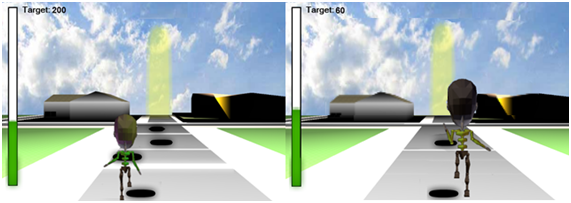
\includegraphics{ch1elderlypeople}
	\caption{Screenshoty HTML5 hry. Vlevo hraje nadaný hráč, vpravo s menší dovedností. \cite{8} }
	\label{ch1elderlypeople}
\end{figure}

\subsubsection{Jogging na dálku}

Ne každého baví běhat po parku samostatně a zároveň může být těžké najít někoho, kdo by si s vámi zaběhal ve stejnou dobu. Řešením může být jogging na dálku (jogging over distance), kdy dva lidé běží ve stejnou dobu, ale každý běží jinde, třeba i v jiném státě. Oba cvičící se dorozumívají přes telefon se sluchátky na hlavě. Povídají si, navzájem se podporují.

Různí lidé mají různou fyzickou kondici a může být problém se navzájem přizpůsobit v běhu tak, aby oba dva jedinci byli přibližně stejně namáhání. Neměla by nastat situace, kdy jeden udýchaně nemůže skoro mluvit a druhému naopak cvičení nic nedává.

V článku Balancing Exertion Experiences \cite{7} popisují svůj přístup k dané problematice. Každý z joggujících partnerů má při sobě chytrý telefon a měřič srdeční frekvence. Na telefonu mají nastavenou svojí ideální, cílovou srdeční frekvenci každý dle své fyzické kondice, případně dle doporučení doktora. Jestliže oba partneři mají srdeční frekvenci relativně stejnou vůči své cílové, pak je vše v pořádku. Partneři mohou běžet několik minut s cílovou srdeční frekvencí, poté se vyhecují, že na chvíli zrychlí a běží např. na 120\% své cílové frekvence. Pokud nastane situace, kdy první partner běží na 80\%, druhý na 110\%, jak vhodně donutit prvního zrychlit a druhého zpomalit? 

Autoři článku přišli se zajímavým řešením. Pomocí sluchátek mohou simulovat vjem, kdy se partneři slyší vedle sebe, kdy jeden slyší druhého před sebou, případně za sebou. Ve výše uvedeném příkladu by partner běžící na 110\% slyšel spoluběžce za ním, což by ho donutilo zpomalit. Opačně partner běžící na 80\% by slyšel toho druhého před sebou a byl by donucen zrychlit, aby se ve výsledku slyšeli co nejlépe, vedle sebe.

\subsection{Zdravotnictví}

Aplikace s adaptivní obtížností mohou pomáhat i nemocným lidem. Lidé po vážných úrazech se mnohdy učí, jak se vrátit zpět do normálního života. Při rehabilitaci lze mnohdy využít i počítačových her, které více motivují ke cvičení. Jestliže je taková hra příliš obtížná, pacient o ní brzy ztratí zájem. To platí i v opačném případě, kdy hra nutí pacienta provádět věci, které již bez problémů zvládá. Z těchto důvodů je velice vhodné obtížnost adaptivně měnit vůči konkrétním pacientům. Příkladem této aplikace je následující podkapitola Rehabilitace po utrpění mozkové mrtvice.

Druhá podkapitola v této sekci popisuje program asistující lidem trpícím demencí při jednoduchých úkolech.

\subsubsection{Rehabilitace po utrpění mozkové mrtvice}

Po cévní mozkové příhodě může dojít k částečnému až k v úplnému ochrnutí některých končetin. Pomocí různých cvičení lze tento dopad zvrátit. Mimo jiné mohou dobře posloužit jednoduché počítačové hry ovládané haptickým zařízením s adaptivním odporem a senzory. Obtížnost hry spočívá především v odporu ovladače a vzdálenosti, kterou musí osoba překonat. Jestliže se obtížnost zvolí špatně, hráč se může brzy nudit, být frustrován. V tom případě hru vypne a může být odrazen od další rehabilitace. Úkolem dynamického vyvažování hry je opět přizpůsobit hru různým lidem s různou rychlostí rehabilitace. \cite{9Pomdp} 

\subsubsection{Pomoc lidem trpícím demencí}

Lidé trpící nemocemi jako je Alzheimerova choroba potřebují pomoci i při běžných úkolech jako je mytí rukou. Tento proces lze rozdělit do několika podúkolů. Puštění vody, namydlení rukou, opláchnutí rukou, vypnutí vody, usušení rukou ručníkem. Někteří pacienti některé z kroků zapomínají, a poté jim je musí aplikace slovně připomenout. Cílem bylo vytvořit aplikaci, která se bude přizpůsobovat dovednostem aktuálního uživatele. Aplikace by neměla připomínat kroky mytí rukou, které pacient zvládne bez nápovědy provést sám. Připomínání všech kroků při každém mytí rukou by mohlo vést k jeho frustraci. \cite{10Dementia} 

\subsection{Výukové programy}

Existuje velké množství vzdělávacích programů a her. Jak takovou hru udělat, aby efektivně vzdělávala úplného začátečníka, ale i již pokročilého uživatele? I zde je prostor pro adaptivní přizpůsobování se programu uživateli. Představme si simulátor výuky v autoškole, kde by se dle schopnostech začínajícího řidiče měnilo prostředí. Na začátku by žák projížděl vesnicemi s minimálním provozem. Jak by se žák zlepšoval, přibýval by provoz, dopravní značky, semafory, vjel by do města apod. Jestliže by jel příliš rychle, v dalším úseku by se objevil retardér atd.

Dále přiblížím dvojici výukových her. První se zaměřuje na na výuky hry na elektrickou kytaru. Druhá má za úkol rozšiřovat slovní zásoby předškolních dětí zábavnou formou.

\subsubsection{Výuka hry na elektrickou kytaru}

Hra Rocksmith má zábavnou formou uživatele naučit hrát na elektronickou kytaru. Oproti Guitar Hero, Rock Band neovládáte hru speciálním plastovým ovladačem, naopak využíváte opravdovou elektrickou kytaru, kterou připojíte přes speciální kabel do USB. Lze využít kytaru zakoupenou se hrou, nebo jakoukoli jinou.

V této výukové hře máte za úkol zahrát na kytaru správné akordy ve správnou chvíli. „Vše začíná jednoduchým brnkáním na jednu notu a pokračuje přes slajdy a příklepy k akordům a dalším složitějším technikám.”\cite{12RocksmithRev} Tímto lze popsat statickou část obtížnosti, ale autoři se zaměřili i na dynamické vyvažování obtížnosti a sami to vyzdvihují ve svém propagačním videu.\cite{13RocksmithVid} Jestliže během hraní uděláte několik chyb po sobě, hra se zjednoduší. Např. místo každého tónu budete hrát pouze každý třetí.

\subsubsection{Rozšiřování slovní zásoby}

Peter Peerdeman se ve své diplomové práci Intelligent Tutoring in Educational Games\cite{14Haas} zabýval využitím DDA u výukových her. Hra Mijn naam is Haas(Moje jméno je Zajíc) je zaměřena na mladší hráče, jež si mají rozšířit svojí slovní zásobu. Hlavní postavou ve hře je zajíc, který se stává průvodcem po hře. Hráč ovládá hru kreslením různých objektů do světa zajíce a hra se mu přizpůsobuje a dle nakreslených objektů vybírá další úkoly. Např. nakreslí-li několik mraků, začne pršet a dalším úkolem je nakreslit deštník, který by ochránil zajíce Haase před zmoknutím.

Hra při zadávání úkolů vhodně vybírá slovíčka dle úrovně hráče. Využívá se databáze 6000 slov, kde každé slovo je ohodnoceno číslem mezi 0 – 100 určující jejich obtížnost. Ohodnocení slova vyjadřuje kolik procent učitelů si myslí, že toto slovo je důležité znát pětiletými dětmi v Holandsku. Lze předpokládat, že slova s hodnotou 90-100 žáci již dobře znají a naopak slova ohodnocená 0 – 30 nejsou důležitá k naučení. Zbytek slov lze rozdělit do šesti úrovní obtížnosti. Obtížnost 1 obsahující slova s hodnotou 80 – 90 až po obtížnost 6 se slovy s hodnotou 30 – 40.

Zadání úkolu vždy obsahuje většinu slov dítěti dobře známých, zbylé tvoří prostor pro učení. Každý úkol má přiřazeno několik různě obtížných synonym a program vybírá nejvhodnější slovo dle úrovně hráče, které několikrát zopakuje v různých větách pro lepší pochopení jeho významu.

\vspace{5mm}

Lze vidět, že DDA má široké spektrum různých aplikací, a proto má smysl se jím zabývat.

\endinput
%%
%% End of file `ch01.tex'.
